\documentclass[12pt, a4paper, onside]{article}
\usepackage[affil-it]{authblk} % author institution
\usepackage{graphicx}

\title{\textbf{Internet of Things: Technologies and Applications -- Lab 4}}
\author{Tran Phong Binh\thanks{Student ID: 110062421}}
\affil{Department of Computer Science, National Tsing Hua University}
\date{\today}

\begin{document}

\maketitle

\section{Part I}
We begin by publishing telemetry events through the gateway, illustrated step by step as follows:
\begin{figure}[h]
  \centering
  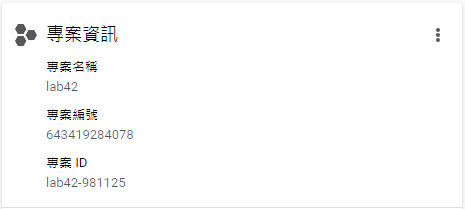
\includegraphics[width=0.6\textwidth]{img/1_cloud_create_project}
  \caption{Create cloud project \texttt{lab42} with ID \texttt{lab42-981125}.}
\end{figure}

\begin{figure}[h]
  \centering
  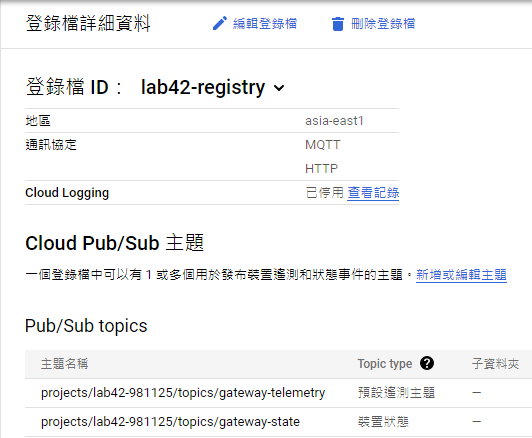
\includegraphics[width=0.6\textwidth]{img/2_cloud_pubsub_topics}
  \caption{Create cloud pub/sub topic \texttt{gateway-telemetry} with device state topic \texttt{gateway-state} under registry ID \texttt{lab42-registry}.}
\end{figure}

\begin{figure}[h]
  \centering
  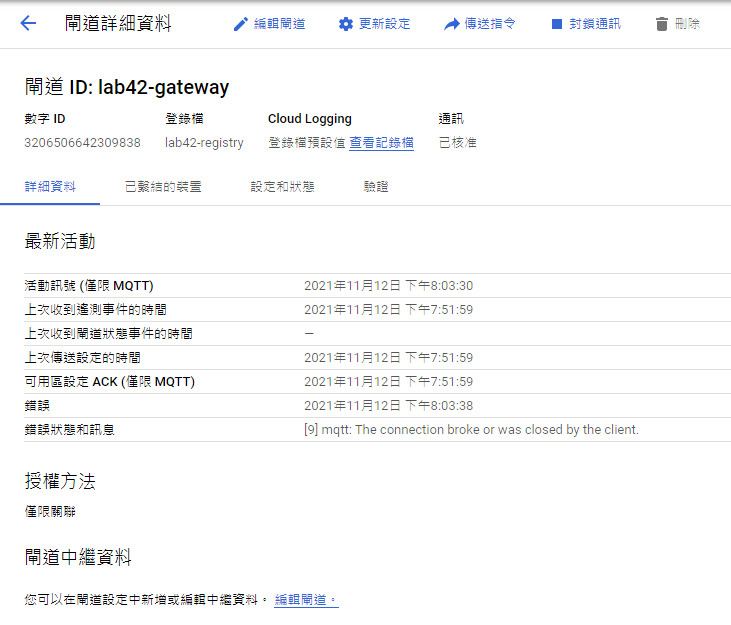
\includegraphics[width=0.6\textwidth]{img/3_cloud_gateway}
  \caption{Create cloud gateway \texttt{lab42-gateway} under \texttt{lab42-registry} using the generated RSA public key.}
\end{figure}

\begin{figure}[h]
  \centering
  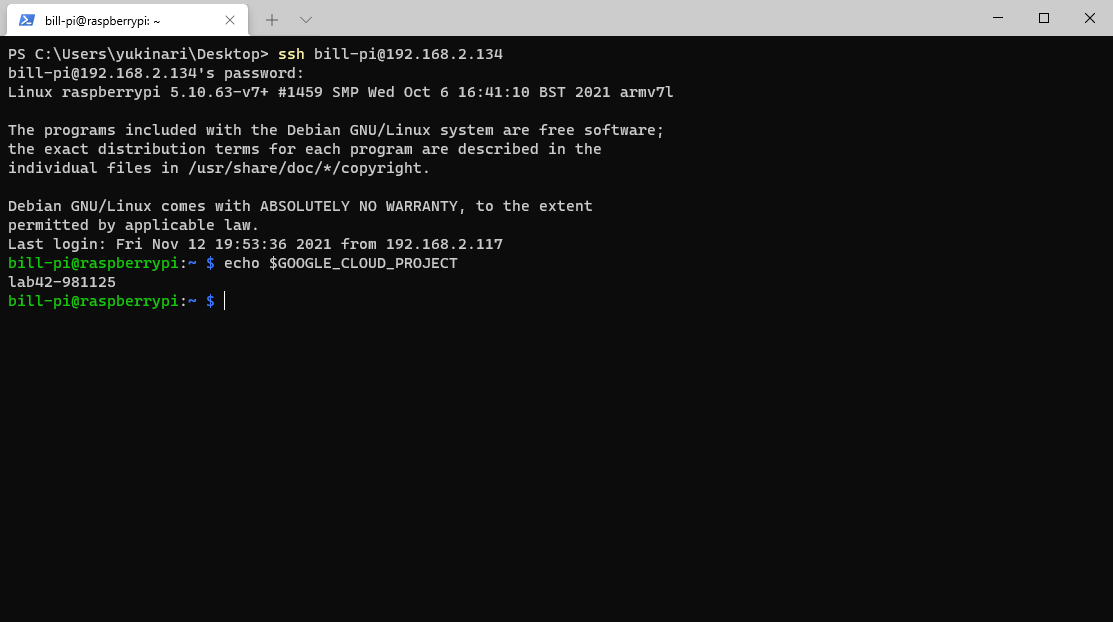
\includegraphics[width=0.6\textwidth]{img/4_local_environment_variable}
  \caption{Set local environment variable \texttt{GOOGLE\_CLOUD\_PROJECT} value to cloud project ID \texttt{lab42-981125}.}
\end{figure}

\begin{figure}[h]
  \centering
  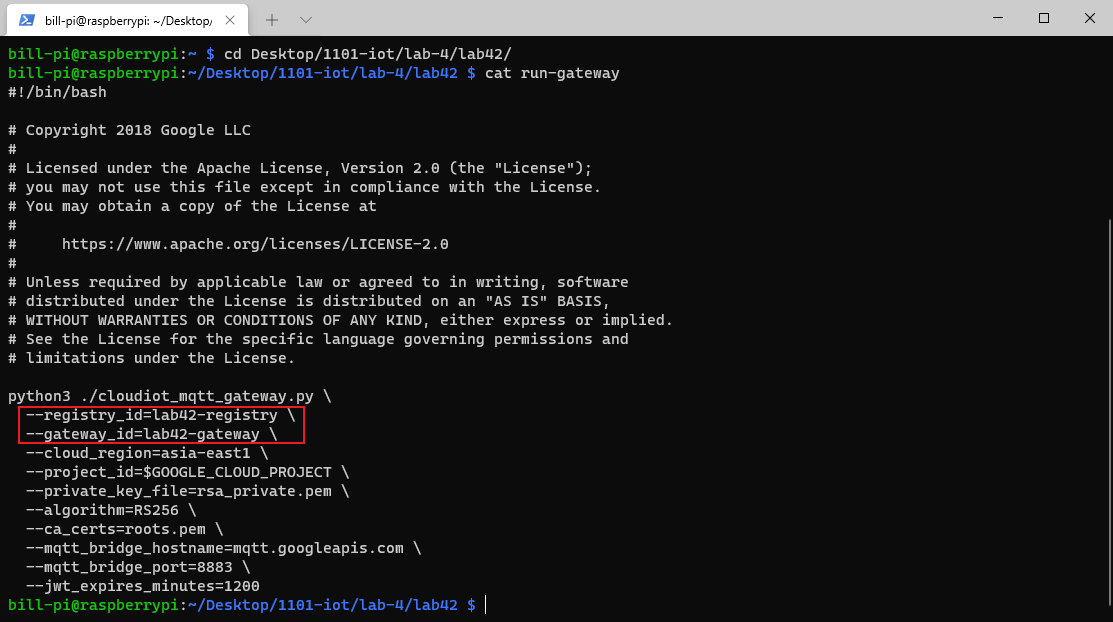
\includegraphics[width=0.6\textwidth]{img/5_local_gateway}
  \caption{Set local registry and gateway ID to \texttt{lab42-registry} and \texttt{lab42-gateway} respectively.}
\end{figure}

\begin{figure}[h]
  \centering
  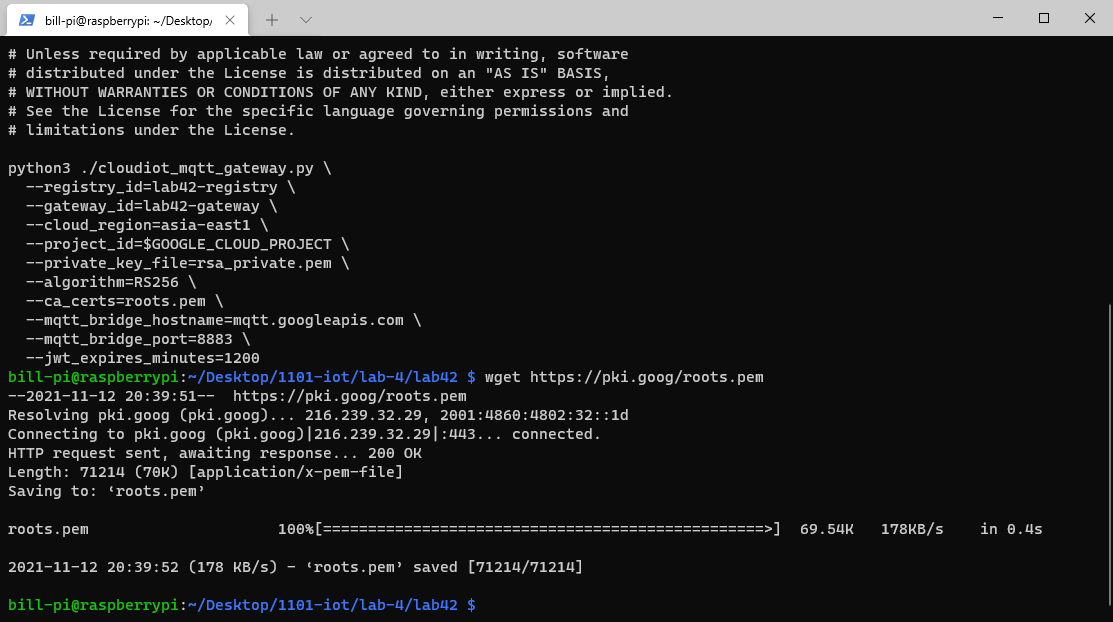
\includegraphics[width=0.6\textwidth]{img/6_local_roots_pem}
  \caption{Get \texttt{roots.pem} from Google API.}
\end{figure}

\begin{figure}[h]
  \centering
  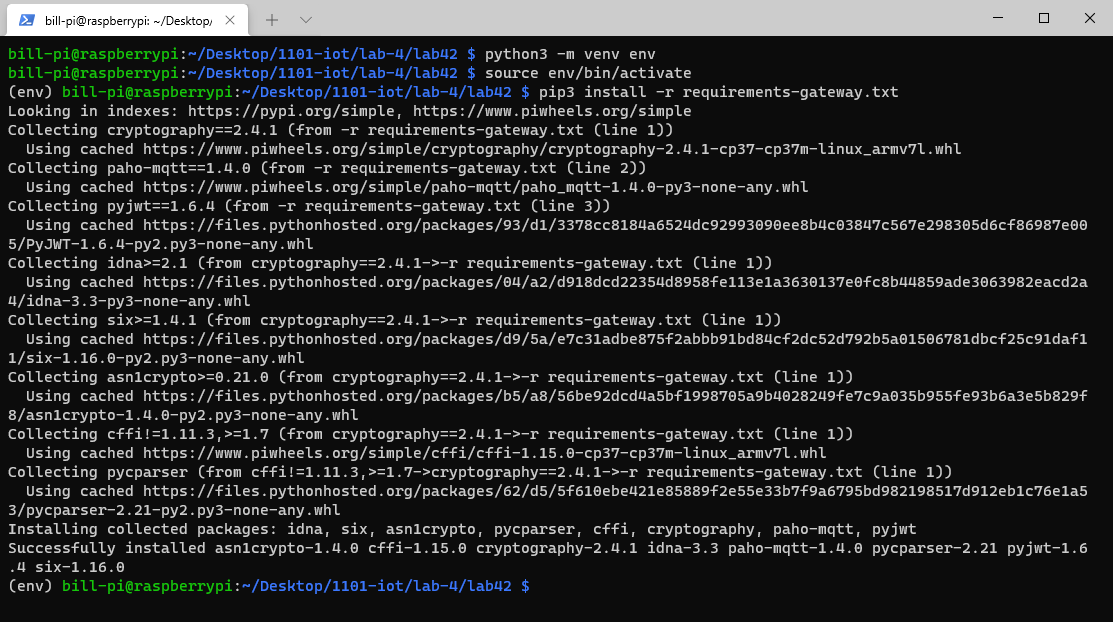
\includegraphics[width=0.6\textwidth]{img/7_local_install_gateway_requirements}
  \caption{Install gateway's requirements.}
\end{figure}

\begin{figure}[h]
  \centering
  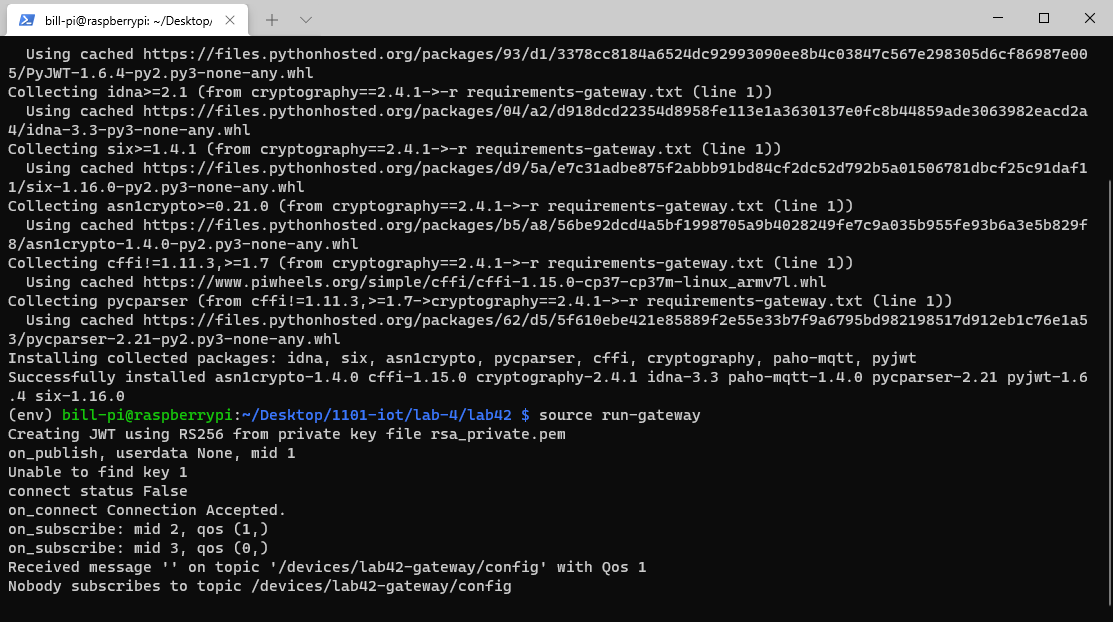
\includegraphics[width=0.6\textwidth]{img/8_local_run_gateway}
  \caption{Run the given gateway program.}
\end{figure}

\begin{figure}[h]
  \centering
  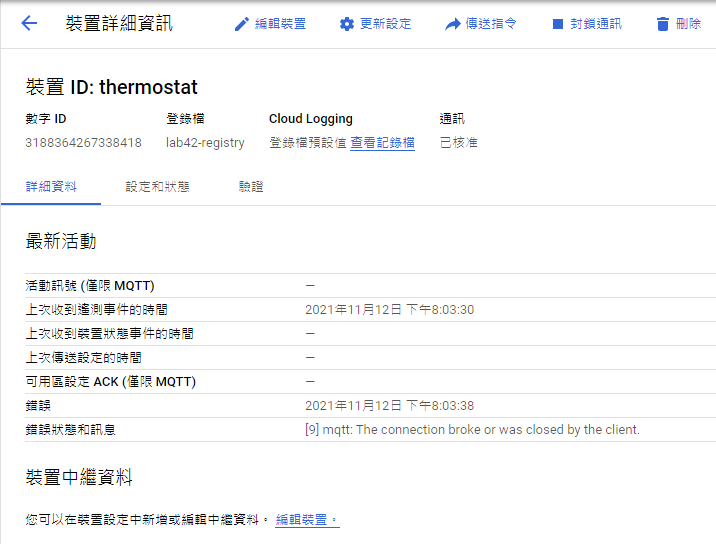
\includegraphics[width=0.6\textwidth]{img/9_cloud_device}
  \caption{Create cloud device with ID \texttt{thermostat} under \texttt{lab42-registry} using the generated RSA public key and add it to gateway \texttt{lab42-gateway}.}
\end{figure}

\begin{figure}[h]
  \centering
  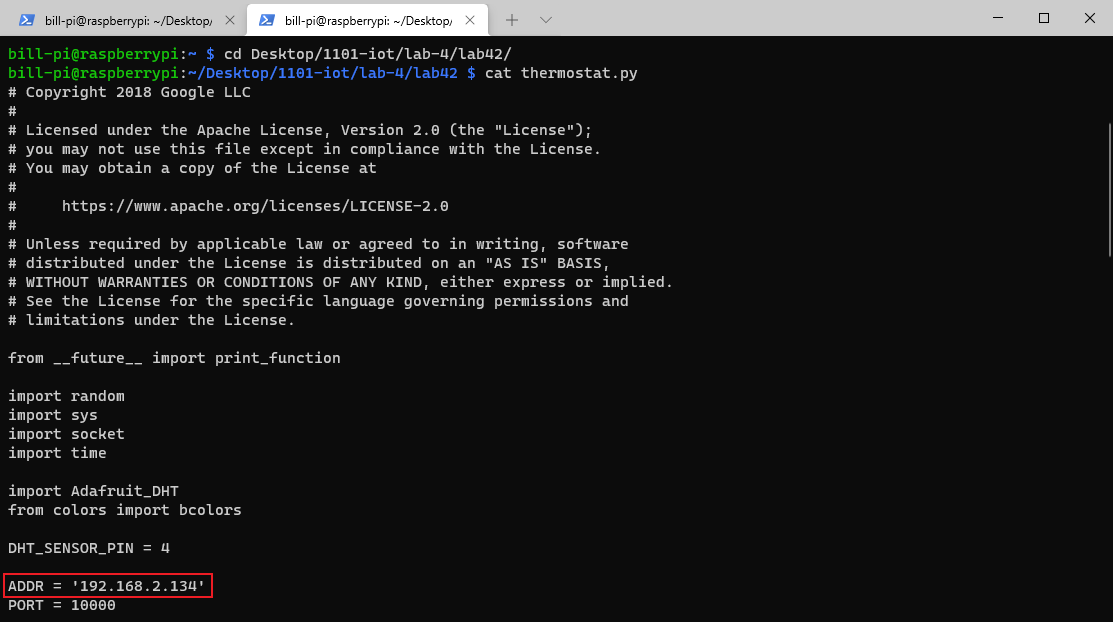
\includegraphics[width=0.6\textwidth]{img/10_local_set_ip}
  \caption{Set IP address in \texttt{thermostat.py} to that of the Raspberry Pi.}
\end{figure}

\begin{figure}[h]
  \centering
  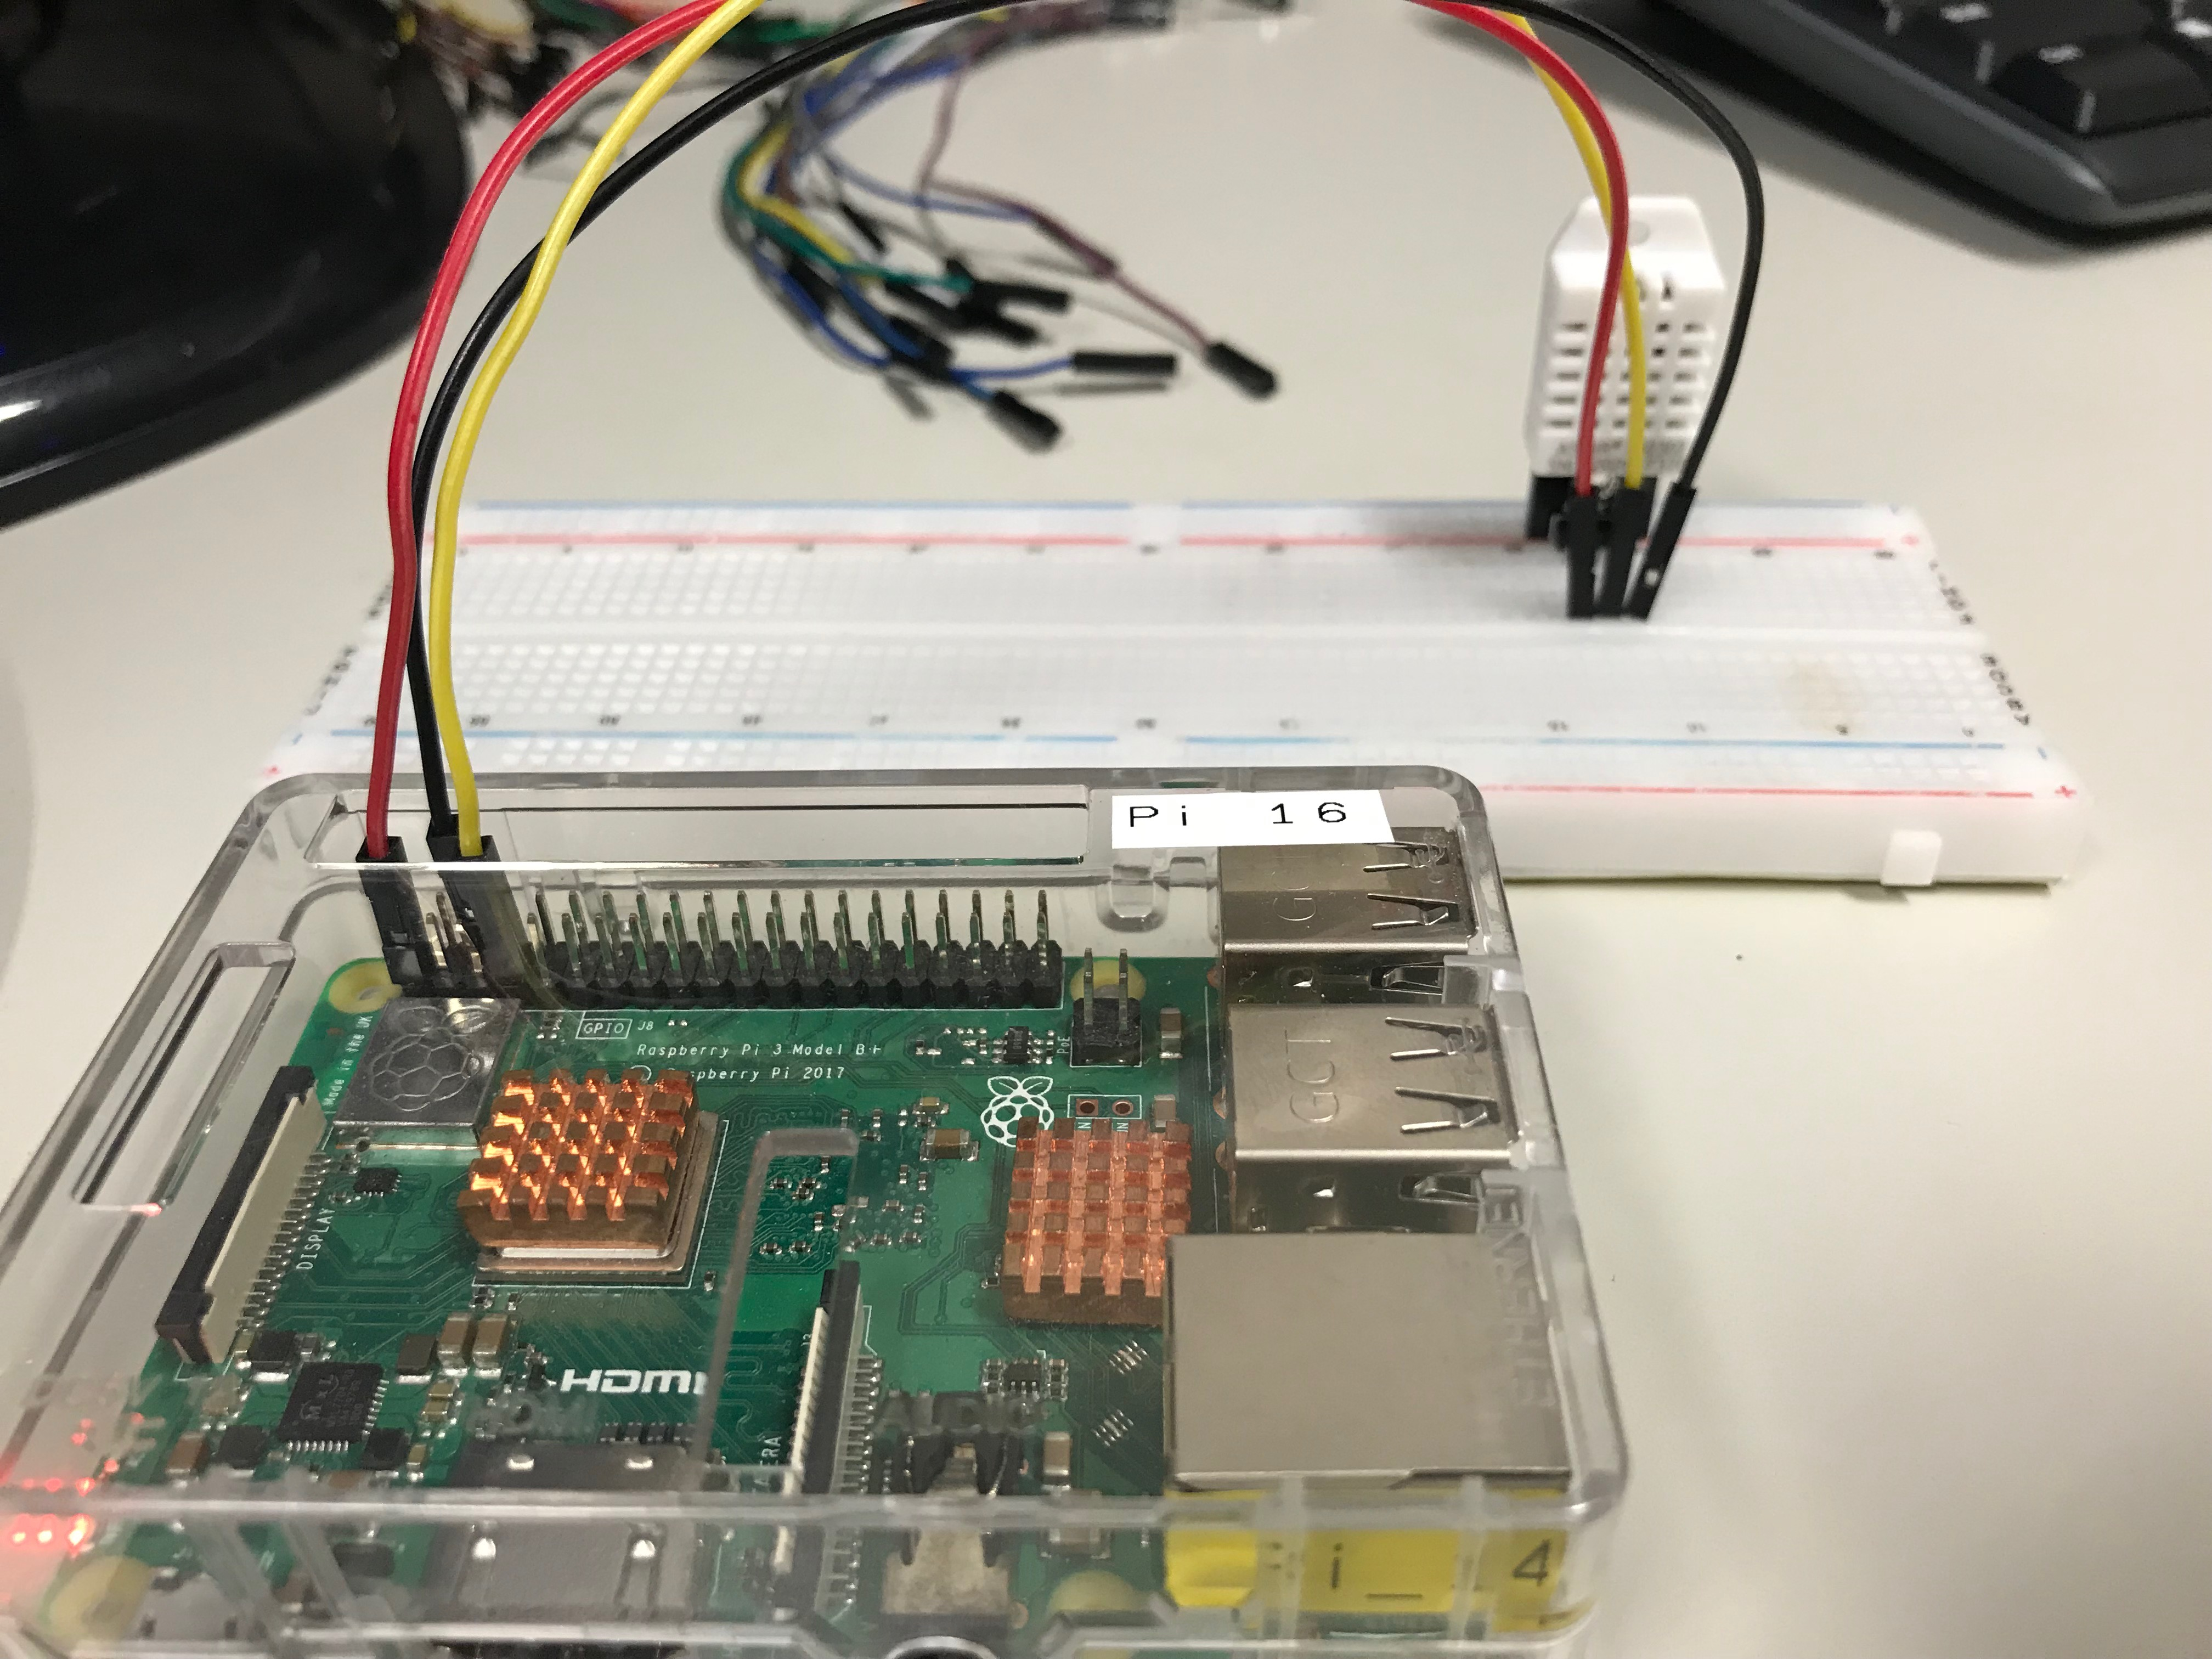
\includegraphics[width=0.6\textwidth]{img/11_local_connect_pin_4}
  \caption{Connect the DHT22 sensor to Raspberry Pi's GPIO pin 4.}
\end{figure}

\begin{figure}[h]
  \centering
  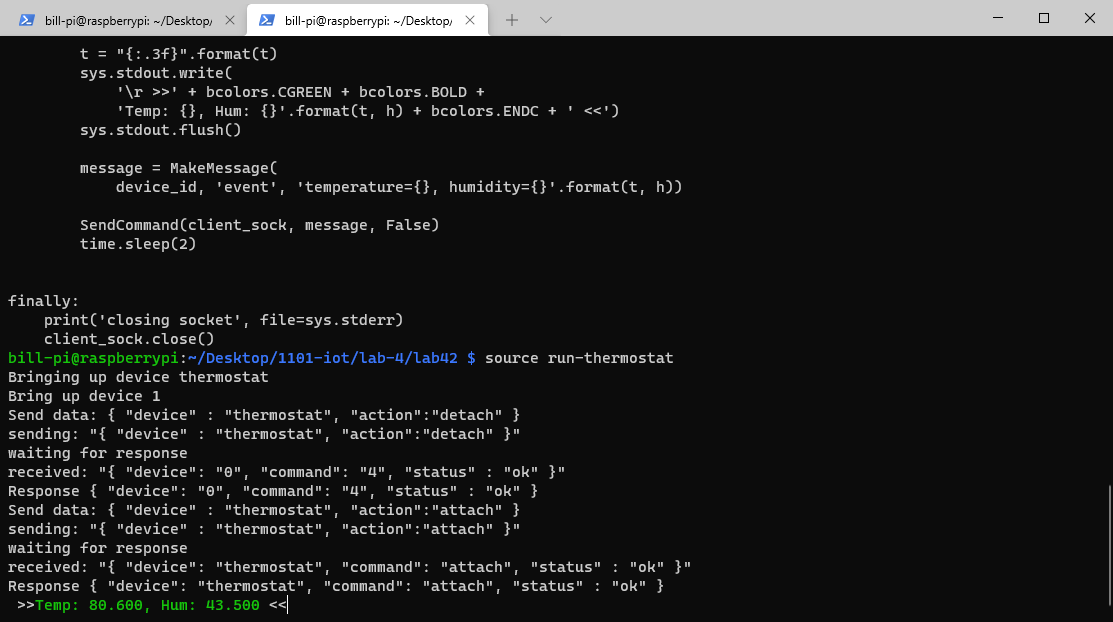
\includegraphics[width=0.6\textwidth]{img/12_local_run_thermostat}
  \caption{Run the given thermostat program.}
\end{figure}
\clearpage

\section{Part II}
In the second part of the experiment, we create a subscription to our telemetry topic to view data:
\begin{figure}[h]
  \centering
  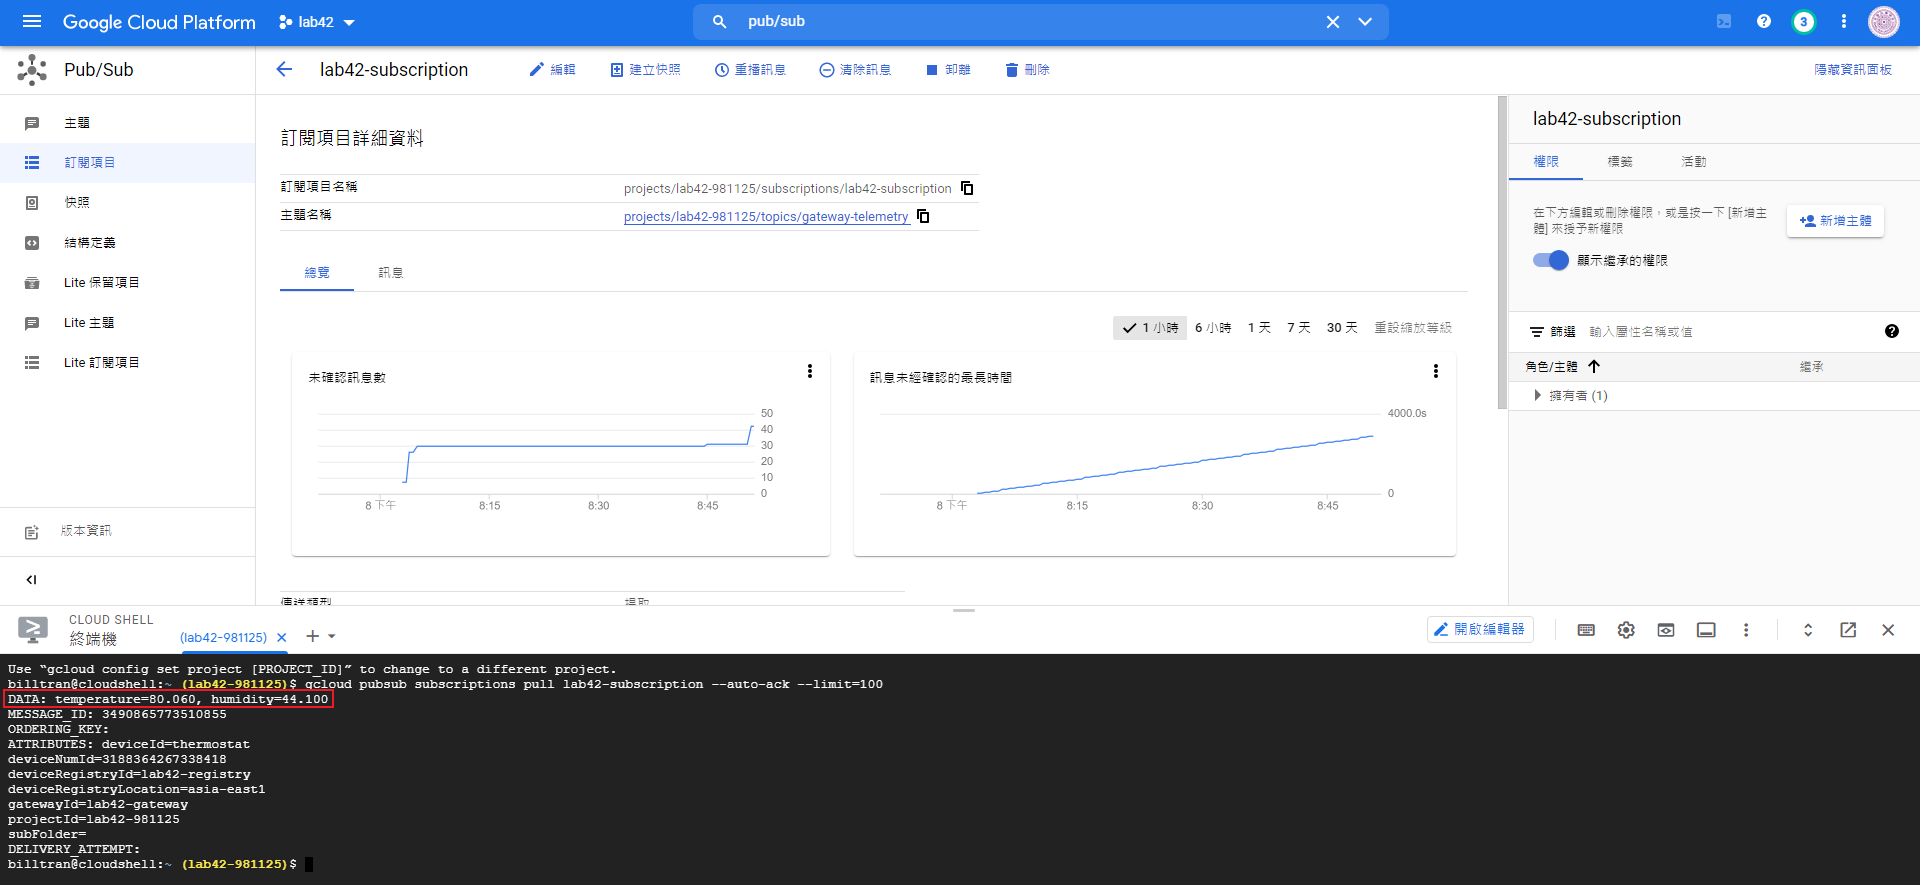
\includegraphics[width=\textwidth]{img/13_cloud_subscription}
  \caption{Execute pull device data command on the Cloud Shell.}
\end{figure}

\end{document}
